\documentclass[tikz, border=10pt]{standalone}
\usepackage{pgfplots}
\pgfplotsset{compat=1.18}
\usetikzlibrary{calc}

\begin{document}

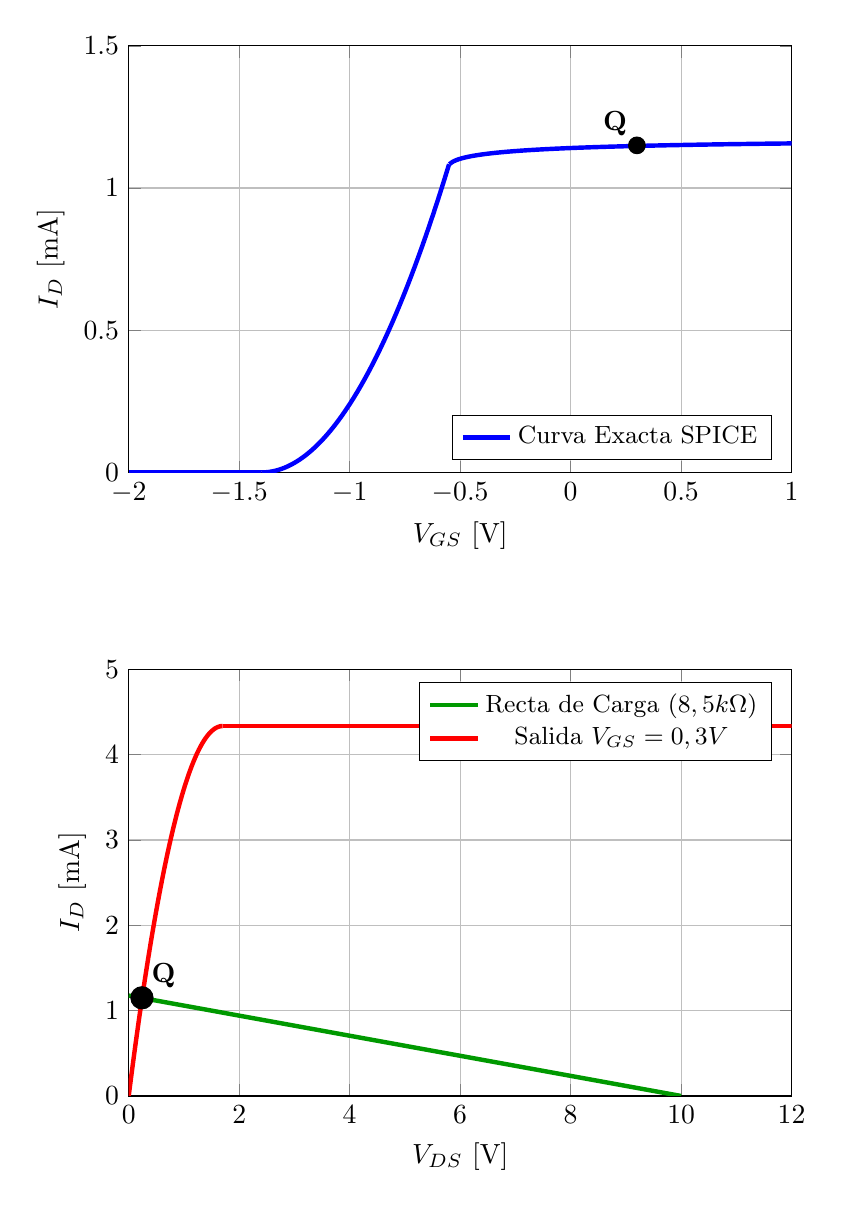
\begin{tikzpicture}
% --- GRÁFICO 1: ENTRADA (TRANSFERENCIA EXACTA CON CARGA) ---
\begin{axis}[
    name=entrada,
    xlabel={$V_{GS}$ [V]}, ylabel={$I_D$ [mA]},
    grid=both, width=10cm, height=7cm,
    xmin=-2, xmax=1, ymin=0, ymax=1.5,
    legend pos=south east,
    legend style={font=\small}
]
    % 1. Zona de Corte
    \addplot[blue, ultra thick, domain=-2:-1.4] {0};
    
    % 2. Zona de Saturación (Vgs desde -1.4V hasta -0.55V)
    % Ecuación de saturación pura: Id = 1.5 * (Vgs + 1.4)^2
    \addplot[blue, ultra thick, domain=-1.4:-0.55, samples=50] {1.5*(x+1.4)^2};
    
    % 3. Zona de Triodo (Vgs > -0.55V, limitado por RD = 8.5k)
    % Graficado paramétricamente usando la ecuación exacta de malla y triodo.
    \addplot[blue, ultra thick, variable=\t, domain=1.0837:1.17, samples=50] 
        ({(\t / (3*(10 - 8.5*\t))) + ((10 - 8.5*\t)/2) - 1.4}, {\t});
    \addlegendentry{Curva Exacta SPICE}

    % PUNTO Q EXACTO
    \addplot[black, mark=*, mark size=3pt] coordinates {(0.3, 1.15)};
    \node[anchor=south east] at (axis cs:0.3, 1.15) {\textbf{Q}};
\end{axis}

% --- GRÁFICO 2: SALIDA Y RECTA DE CARGA EXACTA ---
\begin{axis}[
    name=salida,
    at={($(entrada.south)-(0,2.5cm)$)},
    anchor=north,
    xlabel={$V_{DS}$ [V]}, ylabel={$I_D$ [mA]},
    grid=both, width=10cm, height=7cm,
    xmin=0, xmax=12, ymin=0, ymax=5,
    legend pos=north east,
    legend style={font=\small}
]
    % Recta de Carga: 10V / 8.5k
    \addplot[green!60!black, ultra thick, domain=0:10] {(10 - x) / 8.5};
    \addlegendentry{Recta de Carga ($8,5k\Omega$)}
    
    % Curva de salida para Vgs = 0.3V (Vov = 1.7V)
    % Zona de Triodo: Vds < 1.7V -> Id = 1.5 * (3.4*Vds - Vds^2)
    \addplot[red, ultra thick, domain=0:1.7, samples=100] {1.5*(3.4*x - x^2)};
    % Zona de Saturación: Vds >= 1.7V -> Id = 1.5 * (1.7)^2 = 4.335 mA
    \addplot[red, ultra thick, domain=1.7:12] {4.335};
    \addlegendentry{Salida $V_{GS}=0,3V$}
    
    % PUNTO Q EXACTO (Intersección matemática real)
    \addplot[black, mark=*, mark size=4pt] coordinates {(0.24, 1.15)};
    \node[anchor=south west] at (axis cs:0.24, 1.15) {\textbf{Q}};
\end{axis}
\end{tikzpicture}

\end{document}